\documentclass[letterpaper, 12pt]{article}

\usepackage{titling}
\usepackage[margin=2cm]{geometry}

\usepackage[colorlinks=true]{hyperref}

\usepackage{graphicx}

\usepackage{enumitem}

\usepackage{fontawesome5}

\usepackage{tikz}

% Title (author name and rule)

\newcommand{\name}{
    {\Large\bfseries\MakeUppercase{\theauthor}}
}

\renewcommand{\maketitle}{
    \begin{center}
        \name
    \end{center}
}

% Contact info

\newcommand{\emailnoref}{alejandrogomeznoe@gmail.com}
\newcommand{\email}{\href{mailto:\emailnoref}{\emailnoref}}

\newcommand{\linkedinpage}{\href{https://www.linkedin.com/in/alejandro-g\%C3\%B3mez-bb4239224/}{Alejandro Gómez}}
\newcommand{\githubpage}{\href{https://github.com/algono}{algono}}
\newcommand{\gitlabpage}{\href{https://gitlab.com/algono}{algono}}

% Iconos
\newcommand{\iconoDireccion}{\faIcon{map-marker-alt}}
%\newcommand{\iconoTelefono}{\faPhone}
\newcommand{\iconoTelefono}{\faIcon{phone-alt}}
\newcommand{\iconoEmail}{\faEnvelope}
\newcommand{\iconoNacionalidad}{\faGlobe}
\newcommand{\iconoFechaNacimiento}{\faBirthdayCake}
\newcommand{\iconoDni}{\faIdCard}
\newcommand{\iconoGitHub}{\faGithub}
\newcommand{\iconoGitLab}{\faGitlab}
\newcommand{\iconoLinkedin}{\faLinkedin}

\newcommand{\contactinfo}{
    \begin{minipage}[l]{.25\textwidth}
        \begin{tikzpicture}
        \clip (0,0) circle (2cm) ;
        \node[anchor=center] at (0,0) {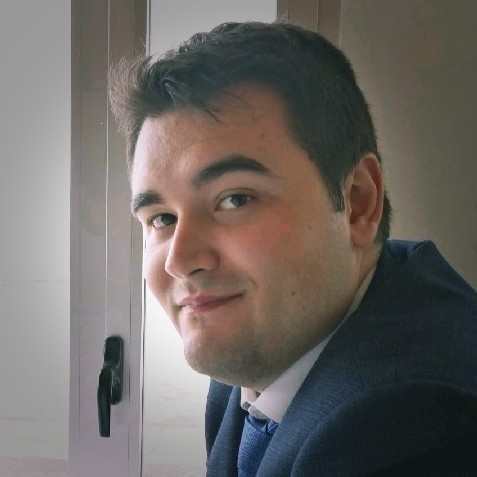
\includegraphics[width=4cm,height=4cm,keepaspectratio]{mi-foto.jpg}};
        \end{tikzpicture}
    \end{minipage}
    \begin{minipage}[r]{.6\textwidth}
        \begin{large}
            \iconoEmail \hspace{.5em} \email \par
            \vspace{12pt}
            \iconoDireccion \hspace{.5em} Mislata, Valencia \par
            \vspace{12pt}
            \iconoLinkedin \hspace{.5em} \linkedinpage \hspace{1em}
            \iconoGitHub \hspace{.5em} \githubpage \hspace{1em} \iconoGitLab \hspace{.5em} \gitlabpage
        \end{large}
    \end{minipage}
    \begin{center}
    Alejandro Gómez es un \textbf{Ingeniero Software},\\\textbf{recién licenciado} en el Grado de \textbf{Ingeniería Informática}\\ por la \textbf{\uni} (2021).
    \end{center}
}

% Other info
\newcommand{\uni}{Universitat Politècnica de València (UPV)}

\newcommand{\fce}{\emph{First Certificate in English - Cambridge}}

% My Grades

\newcommand{\gradesinyear}[2]{
    \begin{itemize}
        \item Nota media: #1
        \item Matrículas de honor: #2
    \end{itemize}
}

\newcommand{\unigrades}[9]{

    \fbox{\begin{minipage}{20em}
        \begin{center}
            \vspace{.7em}

            \textbf{Expediente}
    
            \begin{enumerate}[left=1em,
                label=\arabic*\textdegree curso:]
                \item
                    \gradesinyear{#1}{#2}
                \item
                    \gradesinyear{#3}{#4}
                \item
                    \gradesinyear{#5}{#6}
                \item
                    \gradesinyear{#7}{#8}
            \end{enumerate}

            Nota final (TFG): #9

            \vspace{.1em}
        \end{center}
    \end{minipage}}
    
}

\newcommand{\myunigrades}{
    \unigrades
    {8,3}
    {4}
    {8,1}
    {1}
    {8,3}
    {2}
    {8,4}
    {2}
    {9 (Excelente)}
}

\begin{document}
    
    \title{Curriculum Vitae}
    \author{Alejandro Gómez Noé}
    
    \maketitle

    \contactinfo

    \vspace{8pt}

    \rule{.9\textwidth}{.4pt}

    \section{Conocimientos}

    \renewcommand{\arraystretch}{1.2}
    \begin{Huge}
    \begin{tabular}{cc|c}
        \multicolumn{2}{c}{\textbf{Lenguajes}} & \textbf{Tecnologías}\\[.5ex]
        \faWindows \hspace{.1em} C\# & Dart & \faIcon{node-js} Node.js\\
        \faCoffee \hspace{.1em} Java & \faPython \hspace{.1em} Python & \faIcon{git-alt} Git\\
        TypeScript & \faDatabase \hspace{.1em} SQL & \faDatabase \hspace{.1em} Firebase\\
        \faJs \hspace{.1em} JavaScript & \faLinux \hspace{.1em} Bash & \faMobile \hspace{.1em} Flutter\\
        Haskell & \faMarkdown \hspace{.1em} Markdown & \faUnity Unity\\
        \multicolumn{2}{c|}{\LaTeX} & \faWindows \hspace{.1em} WPF\\\cline{1-2}
        \multicolumn{2}{c|}{\textbf{Herramientas}} & \faDocker \hspace{.1em} Docker\\
        VSCode & \faTrello \hspace{.1em} Trello & \faAmazon \hspace{.1em} Alexa\\
    \end{tabular}
    \end{Huge}
    
    \pagebreak

    \section{Experiencia}

    \begin{center}    
    \textbf{Al Loro - Desarrollador principal}\par
    \vspace{.2em}
    \href{https://github.com/algono/FeedTheParrot-RSS}{Repositorio}\hspace{1em}\href{http://hdl.handle.net/10251/174256}{Memoria}
    \end{center}
    \begin{itemize}
        \item Implementé en solitario una \textbf{skill} para Amazon \textbf{Alexa} como Trabajo de Fin de Grado (\textbf{TFG}), usando \textbf{Node.js} y \textbf{TypeScript}.
        \item Integré la skill con una \textbf{base de datos} en \textbf{Firebase}, creando además una app con \textbf{Flutter} para gestionar las preferencias del usuario.
        \item Diseñé un sistema de autenticación usando servicios de \textbf{AWS} como \textbf{Lambda}, \textbf{DynamoDB} o \textbf{API Gateway}.
    \end{itemize}
    \rule{\textwidth}{.4pt}
    
    \vspace{5pt}
    Los siguientes proyectos participaron en la \href{https://es-es.facebook.com/etsinf/videos/feria-de-proyectos-de-estudiantes-2019/1921312964681641/}{Feria de proyectos (2019)} que organizó la \emph{ETSINF}:

    \vspace{2em}

    \begin{minipage}[l]{.47\textwidth}
        \begin{center}    
        \textbf{Transportify - Desarrollador Jefe}\par
        \vspace{.2em}
        \href{https://github.com/Mobility-Solutions/Transportify}{Repositorio}
        \end{center}
        \begin{itemize}
            \item Lideré un equipo de 8 personas en la creación de una app con \textbf{Flutter} para la asignatura \emph{PIN}.
            \item Desarrollé una serie de componentes para facilitar la integración de la app con la base de datos, diseñada en \textbf{Firebase}.
            \item Gestioné el proyecto mediante \textbf{metodologías ágiles} a través de la plataforma \href{http://www.tuneupprocess.com/}{\textbf{\emph{Worki}}}, desarrollada por nuestro profesor; además del sistema de control de versiones en \textbf{GitHub}, tratando de seguir un flujo de trabajo basado en \textbf{Git flow}.
        \end{itemize}
    \end{minipage}
    \begin{minipage}[r]{.47\textwidth}
        \begin{center}    
        \textbf{Frozen Out - Desarrollador}\par
        \vspace{.2em}
        \href{https://github.com/Mobility-Solutions/Transportify}{Repositorio}
        \end{center}
        \begin{itemize}
            \item Participé en el desarrollo de un videojuego hecho en \textbf{Unity} con \textbf{C\#} como proyecto para la asignatura \emph{IPV}.
            \item Diseñé un \textbf{sistema de diálogos} con soporte para formatos como negrita, cursiva, y distintos colores apoyándome en la librería \href{https://yarnspinner.dev/}{\textbf{\emph{YarnSpinner}}}.
            \item El proyecto continuó sin mí tras la entrega final de la asignatura (Enero de 2020). En Febrero de 2021, \emph{Frozen Out} recibió el \textbf{Premio Especial Compromiso PlayStation} (\href{https://www.inf.upv.es/www/etsinf/es/premio-especial-compromiso-playstation-para-el-videojuego-frozen-out-creado-por-estudiantes-de-la-etsinf-y-la-facultat-de-bb-aa/}{artículo}).
        \end{itemize}
    \end{minipage}

    \section{Educación}

    \subsection{Campus Científicos - 2015}

    Durante el verano de 2015, participé en los \href{https://www.campuscientificos.es/}{Campus Científicos} (organizados por la FECYT y el ministerio de Educación), cursando el proyecto de "Seguridad en Redes e Internet" en la universidad Carlos III de Madrid.

    \subsection{Universidad}

    {\uni}\\
    Grado en Ingeniería Informática, 2021\\

    \myunigrades

    \section{Idiomas}

    \begin{itemize}
        \item \textbf{Español}, nativo
        \item \textbf{Inglés}, nivel \textbf{B2} (\fce)
        \item Valenciano, Bachillerato (sin certificado)
    \end{itemize}

    \section{Actividades}

    \subsection{Mentor - Technovation Challenge}

    Participé como mentor voluntario en el concurso de Iridescent \emph{Technovation Challenge} en su edición del año 2019, en colaboración con el \href{https://cdl.upv.es/american-space}{American Space}, una asociación de la \emph{\uni}.

    \section{Otros}

    \begin{itemize}
        \item Carnet de conducir (tipo B).
    \end{itemize}

\end{document}